\def\year{2018}\relax
%File: formatting-instruction.tex
\documentclass[letterpaper]{article} %DO NOT CHANGE THIS

\usepackage{aaai18}  %Required
\usepackage{times}  %Required
\usepackage{helvet}  %Required
\usepackage{courier}  %Required
\usepackage{url}  %Required
\usepackage{graphicx}  %Required

\usepackage{amsmath,amssymb}
\usepackage{float}
\usepackage{booktabs}
\usepackage{grffile}
\usepackage{color}
\usepackage{xspace}
\usepackage{multirow}
\usepackage{hyperref}
\usepackage{subcaption}


% comments
\newcommand{\yiming}[1]{\textbf{\textcolor{red}{Yiming: #1}}}
\newcommand{\guokun}[1]{\textbf{\textcolor{blue}{Guokun: #1}}}
\newcommand{\peter}[1]{\textbf{\textcolor{violet}{Peter: #1}}}
\newcommand{\hanxiao}[1]{\textbf{\textcolor{green}{Hanxiao: #1}}}

% data sets
\def\electricity{{\sf Electricity}\xspace}
\def\traffic{{\sf Traffic}\xspace}
\def\wind{{\sf Wind}\xspace}
\def\temp{{\sf Temperature}\xspace}
\def\solar{{\sf Solar-Energy}\xspace}
\def\lisf{{\sf LISF}\xspace}
\def\exchange{{\sf Exchange-Rate}\xspace}
\def\stock{{\sf S\&P 500}\xspace}
\def\co{{\sf Gas-CO}\xspace}
\def\methane{{\sf Gas-Methane}\xspace}

% baseline methods
\def\VAR{{\sf VAR}\xspace}
\def\VARMLP{{\sf VAR-MLP}\xspace}
\def\LRidge{{\sf LRidge}\xspace}
\def\LSVR{{\sf LSVR}\xspace}
\def\GP{{\sf GP}\xspace}
\def\TRMF{{\sf TRMF}\xspace}
\def\AR{{\sf AR}\xspace}
\def\RNN{{\sf RNN}\xspace}

\newcommand{\argmin}{\mathop{\mathrm{argmin}}}
\newcommand{\argmax}{\mathop{\mathrm{argmax}}}
\newcommand{\minimize}{\mathop{\mathrm{minimize}}}
\newcommand{\maximize}{\mathop{\mathrm{maximize}}}
\newcommand{\st}{\mathop{\mathrm{subject\,\,to}}}

% shortcuts for symbols
\def\bc{{\boldsymbol c}}
\def\bg{{\boldsymbol g}}
\def\boldf{{\boldsymbol f}}
\def\bq{{\boldsymbol q}}
\def\bu{{\boldsymbol u}}
\def\bv{{\boldsymbol v}}
\def\bw{{\boldsymbol w}}
\def\bx{{\boldsymbol x}}
\def\by{{\boldsymbol y}}
\def\bz{{\boldsymbol z}}
\def\bD{{\boldsymbol D}}
\def\bK{{\boldsymbol K}}
\def\bW{{\boldsymbol W}}
\def\bX{{\boldsymbol X}}
\def\bY{{\boldsymbol Y}}
\def\bZ{{\boldsymbol Z}}

\def\R{{\mathbb{R}}}



\frenchspacing  %Required
\setlength{\pdfpagewidth}{8.5in}  %Required
\setlength{\pdfpageheight}{11in}  %Required
%PDF Info Is Required:
  \pdfinfo{
/Title (2018 Formatting Instructions for Authors Using LaTeX)
/Author (AAAI Press Staff)}
\setcounter{secnumdepth}{0}  


 \begin{document}
% The file aaai.sty is the style file for AAAI Press 
% proceedings, working notes, and technical reports.
%
\title{Modeling Long- and Short-Term Temporal Patterns with Deep Neural Networks}

\author{AAAI Press\\
Association for the Advancement of Artificial Intelligence\\
2275 East Bayshore Road, Suite 160\\
Palo Alto, California 94303\\
}

\iffalse
\author{Guokun Lai}
\affiliation{%
  \institution{Carnegie Mellon University}
}
\email{guokun@cs.cmu.edu}

\author{Wei-Cheng Chang}
\affiliation{%
  \institution{Carnegie Mellon University}
}
\email{wchang2@andrew.cmu.edu}

\author{Yiming Yang}
\affiliation{%
  \institution{Carnegie Mellon University}
}
\email{yiming@cs.cmu.edu}

\author{Hanxiao Liu}
\affiliation{%
  \institution{Carnegie Mellon University}
}
\email{hanxiaol@cs.cmu.edu}
\fi

\maketitle
\begin{abstract}
Multivariate time series forecasting is an important machine learning problem across many domains, including predictions of solar plant energy output, electricity consumption, and traffic jam situation. Temporal data arise in these real-world applications often involves a mixture of long-term and short-term patterns, for which traditional approaches such as Autoregressive models and Gaussian Process may fail. In this paper, we proposed a novel deep learning framework, namely Long- and Short-term Time-series network (LSTNet), to address this open challenge. LSTNet uses the Convolution Neural Network (CNN) to extract short-term local dependency patterns among variables, and the Recurrent Neural Network (RNN) to discover long-term patterns and trends. In our evaluation on real-world data with complex mixtures of repetitive patterns, LSTNet achieved significant performance improvements over that of several state-of-the-art baseline methods.

%Our experiment demonstrates that we assemble the above three parts efficiently, and our model significantly outperform the state-of-art models.
\end{abstract}


\maketitle

\section{Introduction}
\label{sec:intro}

Multivariate time series data are ubiquitous in our everyday life ranging from the prices in stock markets, the traffic flows on highways, the outputs of solar power plants, the temperatures across different cities, and more. In such applications, users are often interested in forecasting new trends or potential hazardous events based on historical observations on time series signals.
%For instance, a better route plan could be devised based on the predicted traffic jam patterns a few hours ahead, and a larger profit could be made with the forecasting of the near-future stock market. %Therefore, in this paper, we focus on the multivariate time series forecasting problem, where the difficulties often grow with the length of time series users wish to forecast ahead.

A major research challenge in multivariate time series forecasting often faces is to capture and leverage the dynamics dependencies among multiple variables.  Specifically, real-world applications often entail a mixture of short-term and long-term repeating patterns, as shown in Figure \ref{fig:tra-ex} which plots the hourly occupancy rate of a freeway.
Apparently, there are two repeating patterns, daily and weekly. The former portraits the morning peaks vs. evening peaks, while the latter reflects the workday and weekend patterns. A successful time series forecasting model should capture both kinds of recurring patterns for accurate predictions. 
%As another example, consider the task of predicting the output of a solar energy farm based on the measured solar radiation by massive sensors over different locations.  The long-term patterns reflect the difference between days vs. nights, summer vs. winter, etc., and the short-term patterns reflect the effects of cloud movements, wind direction changes, etc.  Again, without taking both kinds of recurrent patterns into account, accurate time series forecasting is not possible.  
However, traditional approaches such as the large body of work in autoregressive methods \cite{hamilton1994time,box2015time,zhang2003time,Yu_NIPS_16,li2014forecasting} fall short in this aspect, as most of them do not distinguish the two kinds of patterns nor model their interactions explicitly and dynamically. Addressing such limitations of existing methods is the main focus of this paper, for which we propose a novel framework that takes advantages of recent developments in deep learning research.
%Secondly, there is rich information hidden in the correlation between different variables. For instance, clouds have the most significant influence on the energy output of solar plants. It is plausible to model the relationship between wind directions, the principal factor affecting clouds, and the short-term dependency among the energy output of the solar plants, which is very useful to make accurate forecasts on the future energy productions. Thus how to adequately address the two challenges are essential to develop a reliable multivariate time series forecasting system.
    
\begin{figure}[!t]
	\centering
    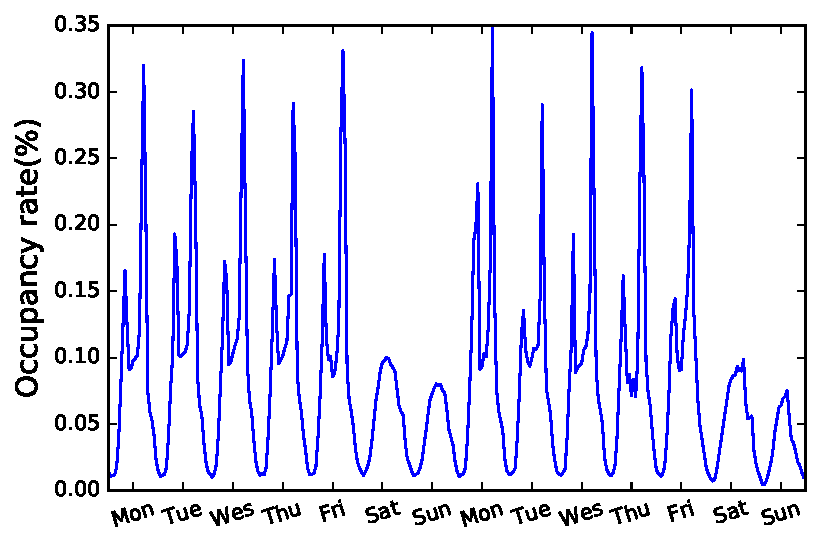
\includegraphics[width=.3\textwidth]{fig/instance.pdf}
    \caption{The hourly occupancy rate of a road in the bay area for 2 weeks}
    \label{fig:tra-ex}
    %\vspace{-1em}
\end{figure}

\begin{figure}[!t]
	\centering
    %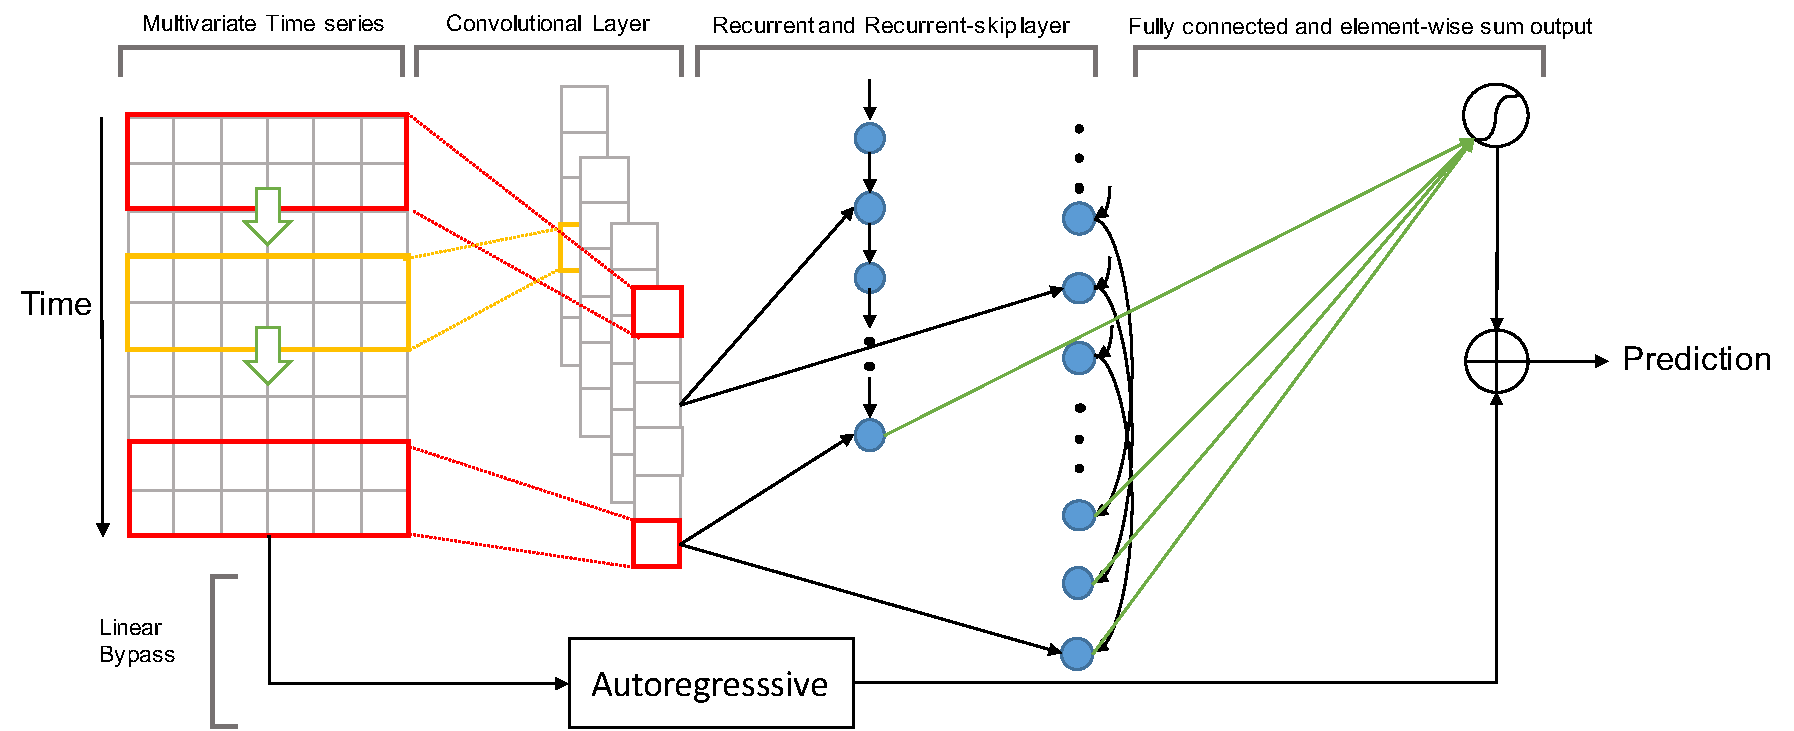
\includegraphics[width=0.75\textwidth]{fig/overview.pdf}
    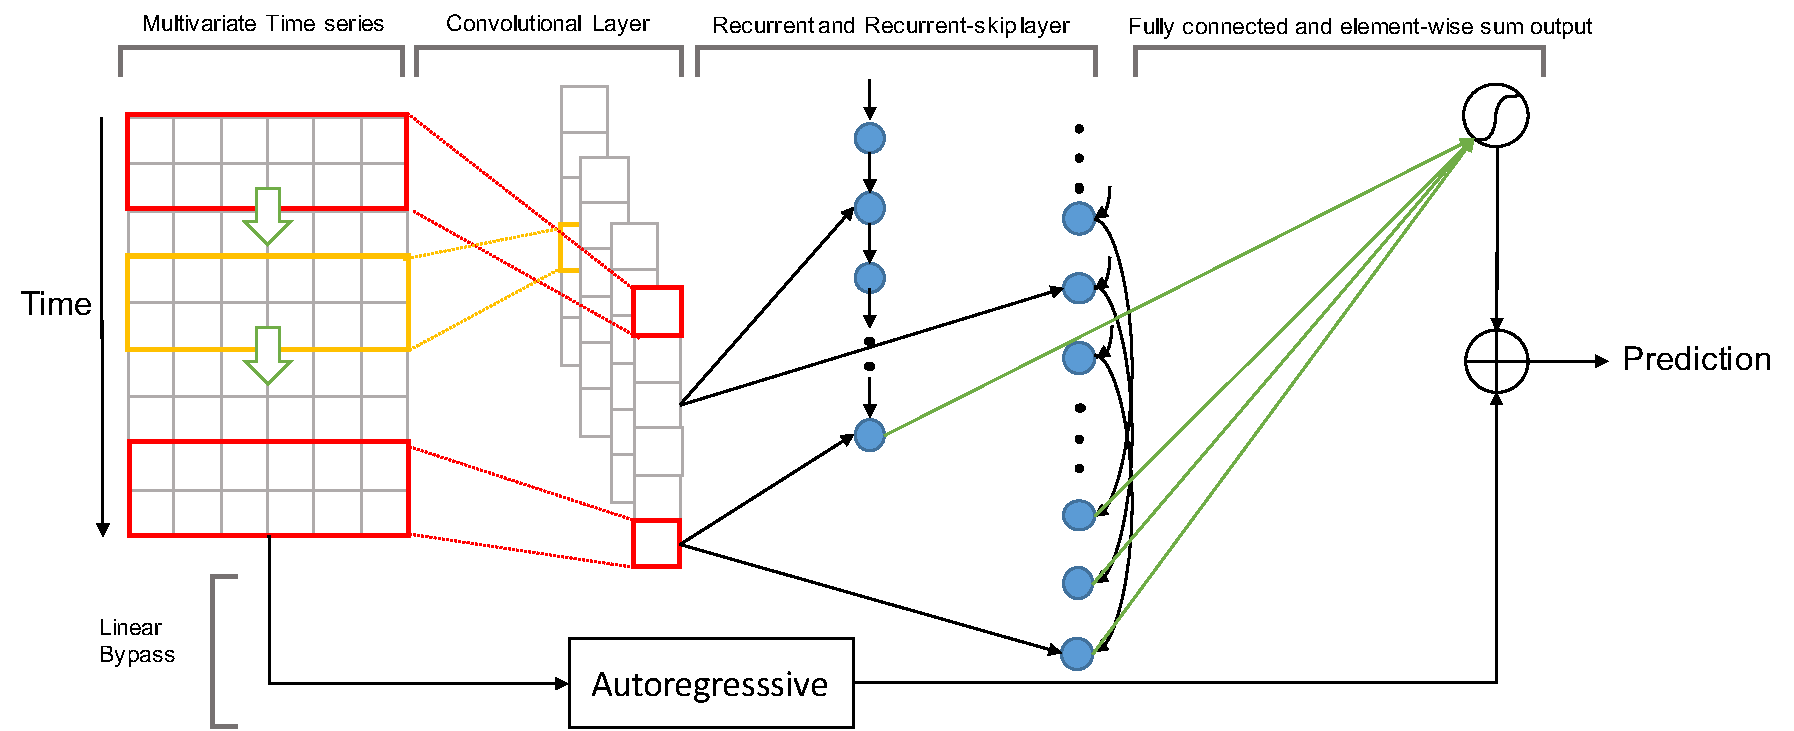
\includegraphics[width=0.475\textwidth]{fig/overview.pdf}
    \caption{An overview of the Long- and Short-term Time-series network (LSTNet)}
    \label{fig:overview}
\end{figure}   
    
%Deep neural networks have been intensively studied in related domains, and made extraordinary impacts on the solutions of a broad range of problems.  The recurrent neural networks (RNN) models \cite{elman1990finding}, for example, have become most popular in recent natural language processing (NLP) research.
%to the analysis of sequential data in temporal nature. %\yiming{Hanxiao et al.: How is "sequential data in temporal nature" different from time series data? Your sentence here would confuse (or mislead) readers because it sounds like that RNN has already been intensively studied in time series forecasting.  It follows that our proposed approach is nothing new but incremental. } 
%Two variants of RNN in particular, namely the Long Short Term Memory (LSTM) \cite{hochreiter1997long} and the Gated Recurrent Unit (GRU) \cite{chung2014empirical}, have significantly improved the state-of-the-art performance in machine translation, speech recognition and other NLP tasks as they can effectively capture the  meanings of words based on the long-term and short-term dependencies among them in input documents  \cite{bahdanau2014neural,hinton2012deep,krizhevsky2012imagenet}.% where the input can be viewed as discrete data streams. RNNs have an outstanding ability to capture long-term temporal dependencies, a desirable property for multivariate time-series forecasting. 
%In the field of computer vision, as another example, convolution neural network (CNN) models \cite{lecun1995convolutional,krizhevsky2012imagenet} have shown outstanding performance by successfully extracting local and shift-invariant features (called "shapelets" sometimes) at various granularity levels from input images.
%saliences from input signals. CNNs are designed for introducing locality to the patterns matched in input data and to enable translational invariance with respect to the exact location, which is the timestamp in time series data. The need of automatically capturing those salient features, or ``shapelets'' over time, makes CNNs suitable for detecting locality patterns in multivariate time series data. 
    
Deep neural networks have received an increasing amount of attention in time series analysis. A substantial portion of the previous work has been focusing on \textit{time series classification}, i.e., the task of automated assignment of class labels to time series input. For instance, RNN architectures have been studied for extracting informative patterns from health-care sequential data \cite{lipton2015learning,che2016recurrent} and classifying the data with respect diagnostic categories.  RNN has also been applied to mobile data, for classifying the input sequences with respect to actions or activities \cite{hammerla2016deep}. CNN models have also been used in action/activity recognition \cite{lea2016temporal,yang2015deep,hammerla2016deep}, for the extraction of shift-invariant local patterns from input sequences as the features of classification models.

Deep neural networks have also been studied for \textit{time series forecasting}, i.e., the task of using observed time series in the past to predict the unknown time series in a look-ahead horizon -- the larger the horizon, the harder the problem. Efforts in this direction range from the early work using naive RNN models \cite{connor1991recurrent} and the hybrid models \cite{zhang1998forecasting,zhang2003time,jain2007hybrid} combining the use of ARIMA \cite{box1970distribution} and Multilayer Perceptron (MLP), to the recent combination of vanilla RNN and Dynamic Boltzmann Machines in time series forecasting \cite{dasgupta2016nonlinear}.

Although the aforementioned work have shed lights on how to use deep neural networks to improve time series analysis, none of them has offered good answers for the important questions below:
\begin{itemize}
 \item How can RNN (LSTM and GRU) and CNN be effectively combined for dynamic modeling of short-term and long-term dependency patterns in multi-variate time series data?
 \item How much can the combined deep learning approach (CNN + RNN) improve the performance of representative autoregressive models? 
 \item Can we further combine the deep learning models (CNN + RNN) and traditional autoregressive models to achieve better performance than that of using each type of the models alone?
\end{itemize}  


Answering the above questions are crucial for improving the state-of-the-art in time series forecasting, and is the main contribution we aim in this paper.  Specifically, we propose a novel deep learning framework, namely Long- and Short-term Time-series Network (LSTNet), as illustrated in Figure \ref{fig:overview}. It leverages the strengths of both the convolutional layer to discover the local dependency patterns among multi-dimensional input variables, and the recurrent layer that captures complex long-term dependencies. A particular recurrent structure, namely Recurrent-skip, is designed for capturing very long-term dependence patterns and making the optimization easier as it utilizes the periodic property of the input time series signals. Finally, the LSTNet incorporates a traditional autoregressive linear model in parallel to the non-linear neural network part; which is similar to a \textit{highway component} \cite{srivastava2015highway}. 
%Adding the linear model to this framework we aim to address a potential weakness of the neural-network model, i.e., when/if the non-linear model is not sufficiently sensitive to the scale changes in input data, the linear model provides a better (more sensitive) alternative. Our evaluation results (Section \ref{sec:ablation}) provide empirical evidence for this assertion. 
% The linear model is sensitive to the scale changing of time series data, which is crucial to some forecasting tasks. To achieve that, we use an autoregressive model as a highway component \cite{srivastava2015highway}. 
%In our experiments on multiple real-world datasets, the proposed method (LSTNet) consistently outperformed other state-of-the-art methods. 
% We also provide a careful ablation study to justify the effectiveness of different components of our deep learning framework for multivariate time series forecasting.

The rest of this paper is organized as follows. Section \ref{sec:related} outlines the related background, including representative auto-regressive methods and Gaussian Process models. Section \ref{sec:model} describe our proposed LSTNet. Section \ref{sec:experiment} reports the evaluation results of our model in comparison with strong baselines on real-world datasets. Finally, we conclude our findings in Section \ref{sec:conclusion}.
       
     
\section{Related Background}
\label{sec:related}

%Peter 
%Time series modeling, also known as linear dynamic system or system identification in the field of control theory \cite{ljung1999system}, aims at the creation of a model based on measured signals. This model can be used, amongst other things, to predict future behavior of the system, to explain interesting structures in the data or to denoise the original time series. 
%In this paper, we are concerned with modeling multivariate time series where a set of observations are associated with multiple output variables. This is in contrast to univariate time series consisting of a set of observations on a single output.
%Time series forecasting models have been applied to a broad raunge of domains, including economic planning and financial markets \cite{azoff1994neural, kim2003financial, granger2014forecasting}, energy consumption \cite{abdel1997forecasting, sfetsos2000comparison}, and various branches of science \cite{jain2007hybrid,reikard2009predicting}. From the perspective of machine learning, time series forecasting can be formulated as a regression task. Existing regression methods for time series forecasting can be categorized into three different ways: linear models, non-linear models, and deep learning models.

One of the most prominent univariate time series models is the autoregressive integrated moving average (ARIMA) model. The popularity of the ARIMA model is due to its statistical properties as well as the well-known Box-Jenkins methodology \cite{box2015time} in the model selection procedure. ARIMA models are not only adaptive to various exponential smoothing techniques \cite{mckenzie1984general} but also flexible enough to subsume other types of time series models including autoregression (AR), moving average (MA) and Autoregressive Moving Average (ARMA). However, ARIMA models, including their variants for modeling long-term temporal dependencies \cite{box2015time}, are rarely used in high dimensional multivariate time series forecasting due to their high computational cost. %Specifically, even the simplest AR model of order $p$ requires $O(Tp^2n^4 + p^3n^6)$ to estimate $O(pn^2)$ parameters. This time complexity is practically infeasible for large number of variables $n$, not to mention other advanced extensions such as ARIMA and seasonal ARIMA.

On the other hand, vector autoregression (VAR) is arguably the most widely used models in multivariate time series
\cite{hamilton1994time,box2015time,lutkepohl2005new} due to its simplicity. VAR models naturally extend AR models to the multivariate setting, which ignores the dependencies between output variables. Significant progress has been made in recent years in a variety of VAR models, including the elliptical VAR model \cite{qiu2015robust} for heavy-tail time series and structured VAR model \cite{melnyk2016estimating} for better interpretations of the dependencies between high dimensional variables, and more. Nevertheless, the model capacity of VAR grows linearly over the temporal window size and quadratically over the number of variables. This implies, when dealing with long-term temporal patterns, the inherited large model is prone to overfitting. To alleviate this issue, \cite{Yu_NIPS_16} proposed to reduce the original high dimensional signals into lower dimensional hidden representations, then applied VAR for forecasting with a variety choice of regularization.

Time series forecasting problems can also be treated as standard regression problems with time-varying parameters. It is therefore not surprising that various regression models with different loss functions and regularization terms are applied to time series forecasting tasks. For example, linear support vector regression (SVR) \cite{kim2003financial,cao2003support} learns a max margin hyperplane based on the regression loss with a hyper-parameter $\epsilon$ controlling the threshold of prediction errors. Ridge regression is yet another example which can be recovered from SVR models by setting $\epsilon$ to zeros. Lastly, \cite{li2014forecasting} applied LASSO models to encourage sparsity in the model parameters so that interesting patterns among different input signals could be manifest. These linear methods are practically more efficient for multivariate time series forecasting due to high-quality off-the-shelf solvers in the machine learning community. Nonetheless, like VARs, those linear models may fail to capture complex non-linear relationships of multivariate signals, resulting in an inferior performance at the cost of its efficiency.

Gaussian Processes (GP) is a non-parametric method for modeling distributions over a continuous domain of functions. This contrasts with models defined by a parameterized class of functions such as VARs and SVRs. GP can be applied to multivariate time series forecasting task as suggested in \cite{roberts2013gaussian}, and can be used as a prior over the function space in Bayesian inference. For example, \cite{frigola2013bayesian} presented a fully Bayesian approach with the GP prior for nonlinear state-space models, which is capable of capturing complex dynamical phenomena. However, the power of Gaussian Process comes with the price of high computation complexity. A straightforward implementation of Gaussian Process for multivariate time-series forecasting has cubic complexity over the number of observations, due to the matrix inversion of the kernel matrix.

%Guokun
%	Recently, Recurrent Neural Networks (RNN)\cite{elman1990finding} and Convolution Neural Networks (CNN)\cite{lecun1995convolutional} have yielded start-of-the-art results across a lot of applications \cite{bahdanau2014neural,hinton2012deep,krizhevsky2012imagenet}. For time series data, researchers have explored them in different related tasks. For instance, the RNN structure has been applied in diagnosis based on extracted patterns out of health-care time series data \cite{lipton2015learning,che2016recurrent} and action/activity detection from mobile data   \cite{hammerla2016deep}. Dasgupta etc.\cite{dasgupta2016nonlinear} has leveraged vanilla RNN and Dynamic Boltzmann Machines for time series prediction and showed results comparable to the LSTM network. And researchers have mainly exploited the CNN structure in action/activity recognition\cite{lea2016temporal,yang2015deep,hammerla2016deep} by utilizing its salient ability to mine the time invariant patterns in time series data.  However, to the best of our knowledge, no work has been conducted to examine how to utilize the RNN(LSTM and GRU) and CNN structures efficiently in the task of multivariate time series forecasting or compare it with the classical time series models.
    
%    Moreover, artificial neural network models had gained great success in univariate time series forecasting problem a decade ago\cite{zhang1998forecasting,zhang2003time,jain2007hybrid}. But researchers only focused on combining ARIMA\cite{box1970distribution} model with Multilayer Perceptron (MLP). However, they only adopted the most naive version among neural network models. Given the tremendous development of the advanced CNN and RNN architectures in these years, it is time to redesigned a more efficient neural network architecture for the time series forecasting task.
    
%Last, another line of research related to time series forecasting is time series classification. \peter{TODO: introduce some time series classification related works.}

\section{Framework}
\label{sec:model}

In this section, we first formulate the time series forecasting problem, and then discuss the details of the proposed LSTNet architecture (Figure \ref{fig:overview}) in the following part. Finally, we introduce the objective function and the optimization strategy.
\subsection{Problem Formulation}
\label{sec:format}

In this paper, we are interested in the task of multivariate time series forecasting. More formally, given a series of fully observed time series signals $\bY = \{\by_1, \by_2, \ldots, \by_T \}$ where $\by_t \in \R^n$, and $n$ is the variable dimension, we aim at predicting a series of future signals in a rolling forecasting fashion. That being said, to predict $\by_{T+h}$ where $h$ is the desirable horizon ahead of the current time stamp, we assume $\{ \by_1, \by_2, \ldots, \by_T \}$ are available. Likewise, to predict the  value of the next time stamp $\by_{T+h+1}$, we assume $\{ \by_1, \by_2, \ldots, \by_T, \by_{T+1}\}$ are available. We hence formulate the input matrix at time stamp $T$ as $X_T = \{ \by_1, \by_2, \ldots, \by_T\} \in \R^{n \times T}$. 

In the most of cases, the horizon of the forecasting task is chosen according to the demands of the environmental settings, e.g. for the traffic usage, the horizon of interest ranges from hours to a day; for the stock market data, even seconds/minutes-ahead forecast can be meaningful for generating returns.

Figure \ref{fig:overview} presents an overview of the proposed LSTnet architecture. The LSTNet is a deep learning framework specifically designed for multivariate time series forecasting tasks with a mixture of long- and short-term patterns. In following sections, we introduce the building blocks for the LSTNet in detail. 

\subsection{Convolutional Component}
The first layer of LSTNet is a convolutional network without pooling, which aims to extract short-term patterns in the time dimension as well as local dependencies between variables. The convolutional layer consists of multiple filters
%and its $k$-th filter is parameterized by $W_k \in \R^{n \times \omega}$ with a bias term $b_k$,
of width $\omega$ and height $n$ (the height is set to be the same as the number of variables). The $k$-th filter sweeps through the input matrix $X$ and produces
\begin{equation}
h_k = RELU(W_k * X + b_k)
\end{equation}
where $*$ denotes the convolution operation and the output $h_k$ would be a vector, and the $RELU$ function is $RELU(x) = \max(0,x)$. We make each vector $h_k$ of length $T$ by zero-padding on the left of input matrix $X$. The output matrix of the convolutional layer is of size $d_c \times T$
where $d_c$ denotes the number of filters.

\subsection{Recurrent Component}
The output of the convolutional layer is simultaneously fed into the Recurrent component and Recurrent-skip component (to be described in subsection \ref{subsec:recurrent-skip}). The Recurrent component is a recurrent layer with the Gated Recurrent Unit (GRU) \cite{chung2014empirical} and uses the $RELU$ function as the hidden update activation function. The hidden state of recurrent units at time $t$ is computed as,

\begin{equation}
\begin{aligned}
r_t &= \sigma(x_tW_{xr} + h_{t-1}W_{hr} + b_r) \\
u_t &= \sigma(x_tW_{xu} + h_{t-1}W_{hu} + b_u) \\
c_t &= RELU(x_tW_{xc} + r_{t}\odot(h_{t-1}W_{hc}) + b_c) \\
h_t &= (1-u_t) \odot h_{t-1} + u_t \odot c_t \\
\end{aligned}
\label{eq:gru}
\end{equation}

where $\odot$ is the element-wise product, $\sigma$ is the sigmoid function and $x_t$ is the input of this layer at time $t$. The output of this layer is the hidden state at each time stamp. While researchers are accustomed to using $\tanh$ function as hidden update activation function, we empirically found $RELU$ leads to more reliable performance, through which the gradient is easier to back propagate. 

\subsection{Recurrent-skip Component}
\label{subsec:recurrent-skip}

The Recurrent layers with GRU \cite{chung2014empirical} and LSTM \cite{hochreiter1997long} unit are carefully designed to memorize the historical information and hence to be aware of relatively long-term dependencies. Due to gradient vanishing, however, GRU and LSTM usually fail to capture very long-term correlation in practice. We propose to alleviate this issue via a novel recurrent-skip component which leverages the periodic pattern in real-world sets. For instance, both the electricity consumption and traffic usage exhibit clear pattern on a daily basis. If we want to predict the electricity consumption at $t$ o'clock for today, a classical trick in the seasonal forecasting model is to leverage the records at $t$ o'clock in historical days, besides the most recent records.
% The intuition here is that signals at the same phase before several periods may have strong correlation to the present signal.
This type of dependencies can hardly be captured by off-the-shelf recurrent units due to the extremely long length of one period (24 hours) and the subsequent optimization issues. Inspired by the effectiveness of this trick, we develop a recurrent structure with temporal skip-connections to extend the temporal span of the information flow and hence to ease the optimization process. Specifically, skip-links are added between the current hidden cell and the hidden cells in the same phase in adjacent periods. The updating process can be formulated as,

\begin{equation}
\begin{aligned}
r_t &= \sigma(x_tW_{xr} + h_{t-p}W_{hr} + b_r) \\
u_t &= \sigma(x_tW_{xu} + h_{t-p}W_{hu} + b_u) \\
c_t &= RELU(x_tW_{xc} + r_{t}\odot(h_{t-p}W_{hc}) + b_c) \\
h_t &= (1-u_t) \odot h_{t-p} + u_t \odot c_t \\
\end{aligned}
\label{eq:rnn-skip}
\end{equation}

where the input of this layer is the output of the convolutional layer, and $p$ is the number of hidden cells skipped through. The value of $p$ can be easily determined for datasets with clear periodic patterns (e.g. $p=24$ for the hourly electricity consumption and traffic usage datasets), and has to be tuned otherwise. In our experiments, we empirically found that a well-tuned $p$ can considerably boost the model performance even for the latter case. Furthermore, the LSTNet could be easily extended to contain variants of the skip length $p$.

We use a dense layer to combine the outputs of the Recurrent and Recurrent-skip components. The inputs to the dense layer include the hidden state of Recurrent component at time stamp $t$, denoted by $h^R_t$, and $p$ hidden states of Recurrent-skip component from time stamp $t-p+1$ to $t$ denoted by $h^S_{t-p+1},h^S_{t-p+2} \ldots, h^S_{t}$. The output of the dense layer is computed as,

\begin{equation}
h^D_t = W^R h^R_t + \sum_{i=0}^{p-1} W^S_{i}h^S_{t-i} + b
\label{eq:dense}
\end{equation}

where $h^D_t$ is the prediction result of the neural network (upper) part in the Fig.\ref{fig:overview} at time stamp $t$.

\subsection{Autoregressive Component}
\label{sec:AR}
Due to the non-linear nature of the Convolutional and Recurrent components, one major drawback of the neural network model is that the scale of outputs is not sensitive to the scale of inputs. Unfortunately, in specific real datasets, the scale of input signals constantly changes in a non-periodic manner, which significantly lowers the forecasting accuracy of the neural network model. A concrete example of this failure is given in Section \ref{sec:ablation}. To address this deficiency, similar in spirit to the highway network \cite{srivastava2015highway}, we decompose the final prediction of LSTNet into a linear part, which primarily focuses on the local scaling issue, plus a non-linear part containing recurring patterns. In the LSTNet architecture, we adopt the classical Autoregressive (AR) model as the linear component. Denote the forecasting result of the AR component as $h^L_{t} \in \R^n$, and the coefficients of the AR model as $W^{ar} \in \R^{q^{ar}}$ and $b^{ar} \in \R$, where $q^{ar}$ is the size of input window over the input matrix. Note that in our model, all dimensions share the same set of linear parameters. The AR model is formulated as follows,
\begin{equation}
h^L_{t,i} = \sum_{k=0}^{q^{ar}-1}W^{ar}_k\by_{t-k,i} + b^{ar}
\end{equation}

The final prediction of LSTNet is then obtained by by integrating the outputs of the neural network part and the AR component:
\begin{equation}
\hat{\bY}_t = h^D_t + h^L_t
\end{equation}
where $\hat{\bY}_t$ denotes the model's final prediction at time stamp $t$.

\subsection{Objective function}
The squared error is the default loss function for many forecasting tasks,
the corresponding optimization objective is formulated as,
\begin{equation}
\minimize_{\Theta}~~~\sum_{t \in \Omega_{Train}} ||\bY_t - \hat{\bY}_{t-h}||_F^2
\label{eq:L2loss}
\end{equation}
where $\Theta$ denotes the parameter set of our model, $\Omega_{Train}$ is the set of time stamps used for training, $||\cdot||_F$ is the Frobenius norm, and $h$ is the horizon as mentioned in Section \ref{sec:format}.
The traditional linear regression model with the square loss function is named as Linear Ridge, which is equivalent to the vector autoregressive model with ridge regularization. However, experiments show that the Linear Support Vector Regression (Linear SVR) \cite{vapnik1997support} dominates the Linear Ridge model in certain datasets. The only difference between Linear SVR and Linear Ridge is the objective function. The objective function for Linear SVR is,

\begin{equation}
\begin{aligned}
\minimize_{\Theta}~~~&\frac{1}{2}||\Theta||_F^2 + C\sum_{t \in \Omega_{Train}} \sum_{i=0}^{n-1} \xi_{t,i} \\
\st~~~& |\hat{\bY}_{t-h,i} - \bY_{t,i}| \le \xi_{t,i} + \epsilon, t \in \Omega_{Train} \\
& \xi_{t,i} \ge 0
\end{aligned}
\label{eq:svr}
\end{equation}
where $C$ and $\epsilon$ are hyper-parameters. Motivated by the remarkable performance of the Linear SVR model, we incorporate its objective function in the LSTNet model as an alternative of the squared loss. For simplicity, we assume $\epsilon=0$\footnote{One could keep $\epsilon$ to make the objective function more faithful to the Linear SVR model without modifying the optimization strategy. We leave this for future study.}, and the objective function above reduces to absolute loss (L1-loss) function as follows:
\begin{equation}
\minimize_{\Theta}~~~\sum_{t \in \Omega_{Train}} \sum_{i=0}^{n-1}|\bY_{t,i} - \hat{\bY}_{t-h,i}|
\label{eq:L1loss}
\end{equation}

In the experiment section, we carefully examine the effectiveness of both objective functions defined in Equation \ref{eq:L2loss} and Equation \ref{eq:L1loss}.

\subsection{Optimization Strategy}
\label{sec:train}

\iffalse
For a time series sequence, the most straightforward training strategy is to treat the problem as a supervision task with an input time series signals and an output time series signals. Its advantage lies in efficient computation, which allows for going though the neural network part one time at each iteration. But the defect is that we only have one training sample. That being said, we cannot apply stochastic gradient decent (SGD) method. Given the highly non-convex nature of neural network objective function, this strategy can easily lead to bad performance, which is stick at the bad local minimal. 
\fi

%In the following, we introduce the way to optimize the MTNN structure. 
Our optimization strategy is the same as that in the traditional time series forecasting model. Supposing the input time series is $\bY_t = \{\by_1, \by_2, \ldots, \by_t \}$, we define a tunable window size $q$, and reformulate the input at time stamp $t$ as $\bX_t = \{\by_{t-q+1}, \by_{t-q+2}, \ldots, \by_t \}$. The problem then becomes a regression task with a set of feature-value pairs $\{\bX_t, \bY_{t+h}\}$, and can be solved by Stochastic Gradient Decent (SGD) or its variants such as Adam \cite{kingma2014adam}.



\section{Evaluation}
\label{sec:experiment}

%In this section, we perform extensive experiments on time series forecasting task of real-world datasets. %\peter{Do we still need toy experiments on synthetic data?}

We conducted extensive experiments with 9 methods (including our new methods) on 4 benchmark datasets for time series forecasting tasks.

\subsection{Methods for Comparison}
\label{sec:baseline}
%The following state-of-the-art methods are considered as comparisons for time series forecasting task. 
The methods in our comparative evaluation are the follows.
\begin{itemize}
    \item \AR stands for the autoregressive model, which is equivalent to the one dimensional VAR model. 
    \item \LRidge is the vector autoregression (VAR) model with L2-regularization
    %, which has been most popular for multivariate time series forecasting.
    \item \LSVR is the vector autoregression (VAR) model with Support Vector Regression loss \cite{vapnik1997support} . 
    %\item \TRMF is the autoregressive model using temporal regularized matrix factorization by \cite{Yu_NIPS_16}.
    \item \GP is the Gaussian Process for time series modeling. \cite{frigola2015bayesian,roberts2013gaussian}
    \item \VARMLP combines Multilayer Perception (MLP) and autoregressive model \cite{zhang2003time}. 
    \item \RNN is the Recurrent Neural Network model using GRU cell. %\peter{TODO}
    \item LST-L1 is our proposed LSTNet model with the absolute loss objective function.
    \item LST-L2 is our proposed LSTNet model with the square loss objective function.
\end{itemize}
For the single output methods above such as \AR, \LRidge, \LSVR and \GP, we just trained $n$ models independently, i.e., one model for each of the $n$ output variables.

\subsection{Metrics}
\label{sec:metrics} 
We consider three evaluation metrics defined as:
\begin{itemize}
	\item Root Relative Squared Error (RSE):
        \begin{equation*}
        RSE = \frac{\sqrt{\sum_{(i,t) \in \Omega_{Test}}(Y_{it} - \hat{Y}_{it})^2}}
        			{\sqrt{\sum_{(i,t) \in \Omega_{Test}} (Y_{it} - \mu(\bY))^2}}
        \end{equation*}
	%\item Relative Absolute Error (RAE) 
  %      \begin{equation*}
  %      RAE = \frac{\sum_{(i,t) \in \Omega_{Test}} |Y_{it} - \hat{Y}_{it}|}
  %      			{\sum_{(i,t) \in \Omega_{Test}} |Y_{it} - \mu(\bY)|}
  %      \label{eq:RAE}
  %      \end{equation*}   
  \item Empirical Correlation Coefficient (CORR)
      \begin{equation*}
      CORR =\frac{1}{n} \sum_{i=1}^n 
        \frac{\sum_t \big(Y_{it} - \mu({\bY}_i)\big) \big(\hat{Y}_{it} - \mu(\hat{\bY}_i)\big)}
      	     {\sqrt{\sum_t \big(Y_{it} - \mu({\bY}_i)\big)^2 \big(\hat{Y}_{it} - \mu(\hat{\bY}_i)\big)^2}}
      \label{eq:Correlation}
      \end{equation*}    
\end{itemize}
where $\mu(\cdot)$ is the mean function and $\bY,\hat{\bY} \in \mathbb{R}^{n\times T}$ are ground true signals and system prediction signals, respectively. RSE, the scaled version of Root Mean Square Error(RMSE), is designed as more interpretable evaluations across different datasets. RSE is lower value the better, while CORR higher value the better.

\subsection{Data}
\label{sec:data}
%We take a broad range of real-world data into consideration while examining the effectiveness of our proposed framework. 
We used four benchmark datasets which are publicly available. We denote time length $T$, number of variables $D$, and 
frequency between two samples $F$.
%Table \ref{tb:data-stats} summarizes the corpus statistics.
\begin{itemize}
    \item \traffic \footnote{\url{http://pems.dot.ca.gov}}: A collection of 48 months (2015-2016) hourly data from the California Department of Transportation. The data describes the road occupancy rates (between 0 and 1) measured by different sensors on San Francisco Bay area freeways. $T=17544$, $D=682$, $F$ is 1 hour. 
    %\item \wind \footnote{\url{https://www.kaggle.com/c/GEF2012-wind-forecasting}}: The wind power generation for $n=7$ wind power farm, measured in every hour. This dataset is from the Wind Forecasting track of Global Energy Forecasting Competition 2012. The data is available for period ranging from the 1st hour of 2009/7/1 to the 12th hour of 2012/6/28.
	%\item \temp \footnote{\url{https://www.ncdc.noaa.gov/crn/qcdatasets.html}}: The Temperature dataset is downloaded from NOAA website, which contains hourly temperature records for 146 major cities in the U.S.A from 2014 to 2016.
    \item \solar \footnote{\url{http://www.nrel.gov/grid/solar-power-data.html}} : the solar power production records in the year of 2006, which is sampled every 10 minutes from 137 PV plants in Alabama State. $T=52560$, $D=137$, $F$ is 10 minutes.
	\item \electricity \footnote{\url{https://archive.ics.uci.edu/ml/datasets/ElectricityLoadDiagrams20112014}}: The electricity consumption in kWh was recorded every 15 minutes from 2012 to 2014, for $n=321$ clients. We converted the data to reflect hourly consumption. $T=26304$, $D=321$, $F$ is 1 hour.
    \item \exchange: the collection of the daily exchange rates of eight foreign countries including Australia, British, Canada, Switzerland, China, Japan, New Zealand and Singapore ranging from 1990 to 2016. $T=7588$, $D=8$, $F$ is 1 day.
\end{itemize}

\iffalse
\begin{table}
	\begin{center}
        \resizebox{0.75\columnwidth}{!}{%
		\begin{tabular}{lrrrrrrrr} 
		\toprule
		Datasets 		 & $T$		 & $D$	& $L$		 \\
		\midrule
		\traffic 		 & 17,544  & 862 	& 1 hour	\\
    \solar			 & 52,560	 & 137	& 10 minutes\\
		\electricity & 26,304  & 321 	& 1 hour	\\
    \exchange		 & 7,588	 & 8		& 1 day		\\
    \bottomrule
		\end{tabular}
        }
        %\vspace{-0.125cm}
        \caption{Dataset Statistics, where $T$ is length of time series, $D$ is number of variables, $L$ is the sample rate.}
		\label{tb:data-stats}
	\end{center}
\end{table}
\fi

All datasets are split into training (60\%), validation (20\%) and test (20\%) set in chronological order. To facilitate future research in multivariate time series forecasting, we publicize all raw datasets and the one after preprocessing in the website
\footnote{\url{https://github.com/laiguokun/multivariate-time-series-data}}.

To examine the existence of long-term and/or short-term repetitive patterns in time series data, we plot autocorrelation graph for some randomly selected variables from the four datasets in Figure \ref{fig:autocorrelation}.
Autocorrelation is the correlation of a signal with a delayed copy of itself as a function of delay, defined as
	$R(\tau) =  \mathbb{E}[(X_t - \mu)(X_{t+\tau} - \mu)] / \sigma^2$
where $X_t$ is the time series signals, $\mu$ is mean and $\sigma^2$ is variance.
%In practice, we consider the empirical unbiased estimator to calculate the autocorrelation.  

In Figure \ref{fig:autocorrelation}, there are repetitive patterns with high autocorrelation in the \traffic, \solar and \electricity datasets, but not in the \exchange dataset. Furthermore, we observe a short-term daily pattern (in every 24 hours) and long-term weekly pattern (in every 7 days) in the \traffic and \electricity dataset, reflecting the expected regularity in highway traffics and electricity consumptions.  On the other hand, we hardly see any repetitive long-term patterns in the \exchange dataset, expect some short-term local continuity. 
These observations suggest for methods capable of leveraging both short-term and long-term repetitive patterns should outperforms on \electricity, \traffic and \solar dataset. In contrast, if the dataset does not contain such patterns (like in \exchange), the advantageous power of those methods may not lead a better performance.
%This key observation is later justified for the reason why our proposed models does not outperform other baseline models on this \exchange dataset.
%In the discussion of sec.\ref{sec:mixture}, the experiment result demonstrates the ability of LSTNet structure to model the complex mixture patterns.  

\begin{figure}[!ht]
\begin{subfigure}{.23\textwidth}
  \centering
  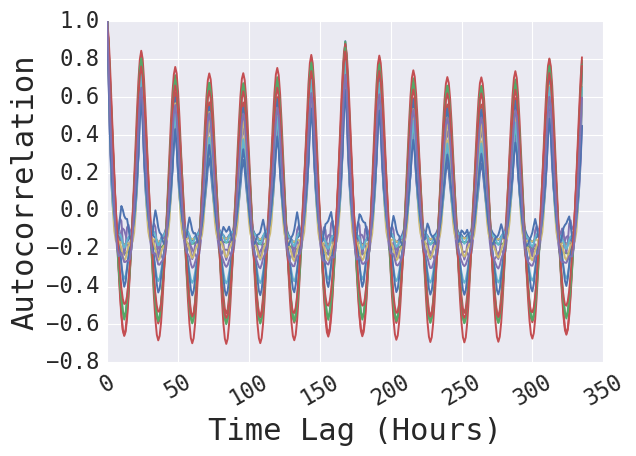
\includegraphics[width=\linewidth]{fig-auto/autocorr_traffic.png}
  \caption{\traffic dataset}
\end{subfigure}
\begin{subfigure}{.23\textwidth}
  \centering
  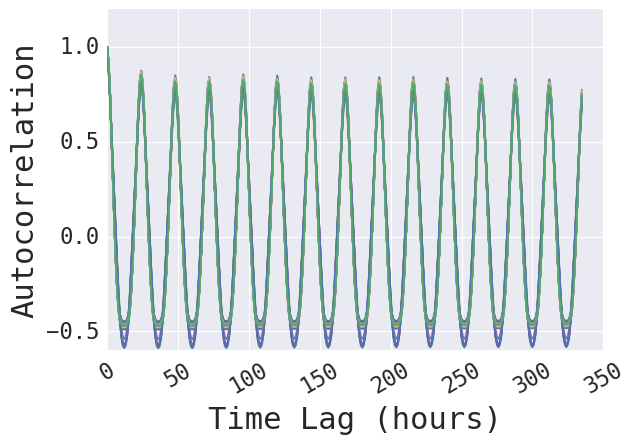
\includegraphics[width=\linewidth]{fig-auto/autocorr_solar.png}
  \caption{\solar dataset}
\end{subfigure}
\begin{subfigure}{.23\textwidth}
  \centering
  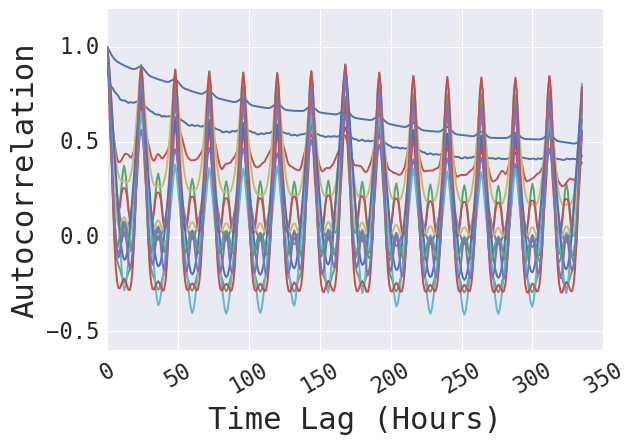
\includegraphics[width=\linewidth]{fig-auto/autocorr_electricity.png}
  \caption{\electricity dataset}
\end{subfigure}
\begin{subfigure}{.23\textwidth}
  \centering
  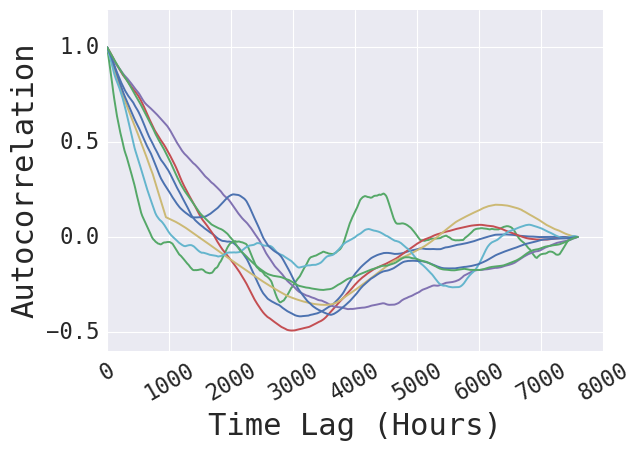
\includegraphics[width=\linewidth]{fig-auto/autocorr_exchange.png}
  \caption{\exchange dataset}
\end{subfigure}
%\vspace{-0.3cm}
\caption{Autocorrelation graphs of some sampled variables.}
\label{fig:autocorrelation}
%\vspace{-0.5cm}
\end{figure}
%\yiming{Peter or Guokun: Make the axis readable!}


\begin{table*}[!ht]
\centering
\resizebox{\textwidth}{!}{
\begin{tabular}{ll|cccc|cccc|cccc|cccc}
\toprule
Dataset &  
        & \multicolumn{4}{c|}{\solar}       & \multicolumn{4}{c|}{\traffic}
        & \multicolumn{4}{c|}{\electricity} & \multicolumn{4}{c}{\exchange}  \\
\midrule
				&
        & \multicolumn{4}{c|}{Horizon} & \multicolumn{4}{c|}{Horizon}
        & \multicolumn{4}{c|}{Horizon} & \multicolumn{4}{c}{Horizon} \\
\midrule
Methods 	& Metrics & 3 & 6 & 12 & 24 & 3 & 6 & 12 & 24 & 3 & 6 & 12 & 24 & 3 & 6 & 12 & 24 \\
\midrule
\multirow{1}{*}{\AR}
  & RSE 
  & 0.2435 & 0.3790 & 0.5911 & 0.8699 
  & 0.5991 & 0.6218 & 0.6252 & 0.6293
  & 0.0995 & 0.1035 & 0.1050 & 0.1054 
  & 0.0228 & 0.0279 & 0.0353 & 0.0445 \\	
  %& RAE 
  %& 0.1846 & 0.3242 & 0.5637 & 0.9221 
  %& 0.4491 & 0.4610 & 0.4700 & 0.4696
  %& 0.0579 & 0.0598 & 0.0603 & 0.0611 
  %& 0.0181 & 0.0224 & 0.0291 & 0.0378 \\
  \textbf{(0)} & CORR 
  & 0.9710 & 0.9263 & 0.8107 & 0.5314 
  & 0.7752 & 0.7568 & 0.7544 & 0.7519
  & 0.8845 & 0.8632 & 0.8591 & 0.8595 
  & 0.9734 & 0.9656 & 0.9526 & 0.9357 \\   
\midrule
\multirow{1}{*}{\LRidge}
  & RSE 
  & 0.2019 & 0.2954 & 0.4832 & 0.7287 
  & 0.5833 & 0.5920 & 0.6148 & 0.6025
  & 0.1467 & 0.1419 & 0.2129 & 0.1280 
  & 0.0184 & 0.0274 & 0.0419 & 0.0675\\
	%& RAE 
  %& 0.1227 & 0.2098 & 0.4070 & 0.6977 
  %& 0.4965 & 0.5115 & 0.5198 & 0.4846
  %& 0.0900 & 0.0933 & 0.1268 & 0.0779 
  %& 0.0144 & 0.0225 & 0.0358 & 0.0602\\
  \textbf{(0)} & CORR 
  & 0.9807 & 0.9568 & 0.8765 & 0.6803 
  & 0.8038 & 0.8051 & 0.7879 & 0.7862
  & 0.8890 & 0.8594 & 0.8003 & 0.8806 
  & 0.9784 & 0.9702 & 0.9543 & 0.9305 \\   
\midrule
\multirow{1}{*}{LSVR}
  & RSE 
	& 0.2021 & 0.2999 & 0.4846 & 0.7300 
  & 0.5740 & 0.6580 & 0.7714 & 0.5909
  & 0.1523 & 0.1372 & 0.1333 & 0.1180 
  & 0.0189 & 0.0284 & 0.0425 & 0.0662 \\
	%& RAE  
  %& 0.1082 & 0.2451 & 0.4362 & 0.6180 
  %& 0.4629 & 0.5483 & 0.7454 & 0.4761
  %& 0.0858 & 0.0816 & 0.0762 & 0.0690
  %& 0.0148 & 0.0231 & 0.0360 & 0.0576 \\
  \textbf{(0)} & CORR 
  & 0.9807 & 0.9562 & 0.8764 & 0.6789 
  & 0.7993 & 0.7267 & 0.6711 & 0.7850 
  & 0.8888 & 0.8861 & 0.8961 & 0.8891 
  & 0.9782 & 0.9697 & 0.9546 & 0.9370 \\   
%\midrule
%\multirow{1}{*}{TRMF}
%  & RSE 
%  & 0.2473 & 0.3470 & 0.5597 & 0.9005 
%  & 0.6708 & 0.6261 & 0.5956 & 0.6442
%  & 0.1802 & 0.2039 & 0.2186 & 0.3656 
%  & 0.0351 & 0.0875 & 0.0494 & 0.0563 \\
%	%& RAE 
%  %& 0.1481 & 0.2165 & 0.3717 & 0.6526
%  %& 0.5887 & 0.5295 & 0.4479 & 0.5256 
%  %& 0.1064 & 0.1175 & 0.1571 & 0.2686 
%  %& 0.0302 & 0.0654 & 0.0464 & 0.0510\\
%  \textbf{(0)} & CORR 
%  & 0.9703 & 0.9418 & 0.8475 & 0.5598
%  & 0.6964 & 0.7430 & 0.7748 & 0.7278 
%  & 0.8538 & 0.8424 & 0.8304 & 0.7471 
%  & 0.9142 & 0.8123 & 0.8993 & 0.8678 \\
\midrule
\multirow{1}{*}{GP}
  & RSE 
	& 0.2259 & 0.3286 & 0.5200 & 0.7973
  & 0.6082 & 0.6772 & 0.6406 & 0.5995
  & 0.1500 & 0.1907 & 0.1621 & 0.1273 
  & 0.0239 & 0.0272 & 0.0394 & 0.0580 \\
	%& RAE 
  %& 0.1419 & 0.2189 & 0.4095 & 0.7599
  %& 0.5148 & 0.5759 & 0.5316 & 0.4829
  %& 0.0907 & 0.1137 & 0.1043 & 0.0776
  %& 0.0230 & 0.0239 & 0.0355 & 0.0547 \\
  \textbf{(0)} & CORR 
  & 0.9751 & 0.9448 & 0.8518 & 0.5971
  & 0.7831 & 0.7406 & 0.7671 & 0.7909
  & 0.8670 & 0.8334 & 0.8394 & 0.8818
  & 0.8713 & 0.8193 & 0.8484 & 0.8278\\
\midrule
\multirow{1}{*}{VARMLP}
  & RSE 
	& 0.1922 & 0.2679 & 0.4244 & 0.6841 
  & 0.5582 & 0.6579 & 0.6023 & 0.6146 
  & 0.1393 & 0.1620 & 0.1557 & 0.1274
  & 0.0265 & 0.0304 & 0.0407 & 0.0578\\
  %& RAE  
  %& 0.1051 & 0.1635 & 0.3102 & 0.6084 
  %& 0.4510 & 0.5434 & 0.4947 & 0.5474
  %& 0.0970 & 0.1171 & 0.1261 & 0.0883
  %& 0.0244 & 0.0268 & 0.0356 & 0.0520 \\
  \textbf{(0)} & CORR 
  & 0.9829 & 0.9655 & 0.9058 & 0.7149 
  & 0.8245 & 0.7695 & 0.7929 & 0.7891
  & 0.8708 & 0.8389 & 0.8192 & 0.8679
  & 0.8609 & 0.8725 & 0.8280 & 0.7675 \\
\midrule
\multirow{1}{*}{RNN-GRU}
  & RSE 
  & 0.1932 & 0.2628 & 0.4163 & 0.4852 
  & 0.5358 & 0.5522 & 0.5562 & 0.5633 
  & 0.1102 & 0.1144 & 0.1183 & 0.1295 
  & 0.0192 & 0.0264 & 0.0408 & 0.0626\\
  %& RAE 
  %& 0.0986 & 0.1389 & 0.2226 & 0.2822 
  %& 0.3596 & 0.3747 & 0.3890 & 0.3965
  %& 0.0765 & 0.0806 & 0.0836 & 0.0829 
  %& 0.0157 & 0.0224 & 0.0372 & 0.0572\\
  \textbf{(0)} & CORR 
  & 0.9823 & 0.9675 & 0.9150 & 0.9823
  & 0.8511 & 0.8405 & 0.8345 & 0.8300
  & 0.8597 & 0.8625 & 0.8472 & 0.8651 
  & 0.9786 & 0.9712 & 0.9531 & 0.9223\\
\midrule
\multirow{}{*}{LSTNet-Skip}
  & RSE 
  & 0.1843 & 0.2559 & 0.3254 & 0.4636 
  & 0.4849 & 0.4995 & 0.5110 & 0.5221 
  & 0.0864 & 0.0931 & 0.1007 & 0.1060 
  & 0.0232 & 0.0302 & 0.0382 & 0.0570\\
  %& RAE 
  %& 0.0923 & 0.1360 & 0.1894 & 0.3484 
  %& 0.3163 & 0.3307 & 0.3443 & 0.3509
  %& 0.0519 & 0.0563 & 0.0572 & 0.0571 
  %& 0.0189 & 0.0253 & 0.0313 & 0.0498\\
  \textbf{(0)} & CORR 
  & 0.9843 & 0.9690 & 0.9467 & 0.8870
  & 0.8721 & 0.8645 & 0.8576 & 0.8552
  & 0.9283 & 0.9135 & 0.9077 & 0.9119 
  & 0.9746 & 0.9670 & 0.9517 & 0.9314\\
%\midrule                                                
%\multirow{2}{*}{LST-L2}
%  & RSE 
%	& 0.1988 & 0.2726 & 0.3780 & 0.4928
%	& \textbf{0.4777} & \textbf{0.4893} & \textbf{0.4950} & \textbf{0.4973}
%  & 0.0967 & 0.1013 & 0.1017 & 0.1010
%	& 0.0226 & 0.0280 & 0.0356 & 0.0449\\
%	& RAE 
%	& 0.1126 & 0.1796 & 0.2593 & 0.3124
%	& 0.3541 & 0.3830 & \textbf{0.3749} & \textbf{0.3887}
%  & 0.0581 & 0.0598 & 0.0601 & 0.0600
%	& 0.0180 & 0.0226 & 0.0296 & 0.0378\\
%  \textbf{(10)} & CORR 
%  & 0.9826 & 0.9639 & 0.9255 & 0.8670 
%  & \textbf{0.8715} & \textbf{0.8627} & \textbf{0.8614} & \textbf{0.8588}
%  & 0.8941 & 0.8764 & 0.8765 & 0.8848
%  & 0.9735 & 0.9658 & 0.9511 & 0.9354\\ 
                                                
\bottomrule
\end{tabular}
}
\caption{Results summary: 1) bold face indicates the best result of each column in a particular metric; and 2) the total number of bold-faced results of each method is listed under the method name within parentheses. }
\label{tb:result}
%\vspace{-0.5cm}
\end{table*}




\subsection{Experimental Details}
%\peter{TODO:modify description of window size and add GP, TRMF}
We conduct grid search over all tunable hyper-parameters on the validation set for each method and dataset. Specifically, all methods share the same grid search range of the window size $q$ ranging from $\{2^0,2^1,\ldots,2^9\}$ if applied. For \LRidge and \LSVR, the regularization coefficient $\lambda$ is chosen from $\{2^{-10}, 2^{-8}, \ldots, 2^{8}, 2^{10}\}$. For \GP, the RBF kernel bandwidth $\sigma$ and the noise level $\alpha$ are chosen from $\{2^{-10}, 2^{-8}, \ldots, 2^{8}, 2^{10}\}$. For \TRMF, the hidden dimension is chosen from $\{2^2, \ldots, 2^6\}$ and the regularization coefficient $\lambda$ is chosen from $\{0.1, 1, 10\}$.  For LSTNet, we adopted the hidden dimension of the Recurrent and Convolutional layer is chosen from $\{50,100,200\}$, and $\{20,50,100\}$ for Recurrent-skip layer. The skip-length $p$ of Recurrent-skip layer is set as 24 for the \traffic and \electricity dataset, and tuned range from $2^1$ to $2^6$ for the \solar and \exchange datasets. The regularization coefficient of the AR component is chosen from $\{0.1,1,10\}$ to achieve the best performance. The Adam\cite{kingma2014adam} algorithm is utilized to optimize the parameters of our model.


\subsection{Main Results}
\label{sec:result}

%Following the problem format in Sec.\ref{sec:format}, we perform the time series forecasting with $horizon = \{3,6,12,24\}$ across all datasets. The horizons are chosen by considering the real demanding of different applications. First, for traffic usage and electricity consumption, people are more care about the situation in next several hours to a day. In the energy output of solar farms, the prediction dozens of minutes ahead are more valuable compared to the long horizon. Because, researchers usually leverage satellite cloud pictures, which have a low refresh frequency, to forecast output in next half or a day. In the economic area, people only demand the prediction few seconds ahead, but the minimum granularity of public economic datasets is a day. However, it is still a good example of the time series signals without the repetitive patterns.   

Table \ref{tb:result} summarizes the evaluation results. We set $horizon = \{3,6,12,24\}$, which means the horizons was set from 3 to 24 hours for the forecasting over the \electricity and \traffic data, from 30 to 240 minutes over the \solar data, and from 3 to 24 days over the \exchange data. The larger the horizons, the harder the prediction tasks. The best result for each (data, metric) pair is highlighted in bold face in this table.  The total count of the bold-faced results is 28 for LST-L1 (one version of the proposed LSTNet), 10 for LST-L2 (the other version of our LSTNet), 5 for AR, 4 for LRidge, and between 0 to 2 for the rest of the methods.  

Clearly, LSTNet has the dominating performance on the first three datasets (\electricity, \solar and \traffic), especially in the settings with the large horizon. In the $horizon=24$ settings, LSTNet model improves the best state-of-the-art result by $35\%$ in \solar, $20\%$ in \traffic and $5\%$ in \electricity dataset in RSE evaluation metric. But it is slightly worse than AR and LRidge on the \exchange dataset. Why?  Recall that in Section \ref{sec:data} and Figure  \ref{fig:autocorrelation} we used the autocorrelation curves of these datasets to show the existence of  repetitive patterns in the \solar, \traffic and \electricity datasets but not in \exchange.  The current results provide empirical evidence for the success of LSTNet models in modeling long-term and short-term dependency patterns when they do occur in data.  Otherwise, LSTNet performed comparably  with the better ones (AR and LRidge) among the representative baselines.  The robustness of LSTNet is also due to its inclusion of the autoregressive model as a component, which we will discuss further in next section.


%show our proposed models outperform baseline algorithms in all evaluation metrics and in all settings of \electricity, \solar and \traffic datasets, except $horizon = 3$ of \solar data, which is slightly below the \VARMLP model. In the most difficult situation of each dataset, where $horizon = 12,24$, our models enhance the state-of-the-art results by 5\% to 30\%. The outstanding accuracy in long-horizon forecasting settings gives the evidence of the ability of the LSTNet to model the mixture of sophisticate patterns. However, in \exchange dataset,  because of lacking the dependencies in the time dimension, LSTNet structure cannot enhance the state-of-the-art result. But they are still at the same level.

Compared the results of univariate AR with that of the multivariate baseline methods, we see that in some datasets, i.e. \solar and \traffic, the multivariate is stronger, but weaker otherwise, which means that the richer input information would causes overfitting in the traditional multivariate approaches. In contrast, the LSTNet has robust performance in different situations, partly due to its  autoregressive component, which we will discuss further in Section \ref{sec:ablation}.

%In \electricity dataset, the performance of \LSVR model dominates the \LRidge model. It is the motivation that we try to leverage the L1-loss objective function in the LSTNet architecture. Across different datasets, the LST-L1 gains better result in \electricity and \solar datasets, and the LST-L2 is better in \traffic. So it is determined by the dataset that which one, L1 or L2, is the better objective function choice for our framework.




\subsection{Ablation Study}
\label{sec:ablation}
%To demonstrate the efficiency of our framework design, a careful ablation study is conducted. Specifically, we remove each component one at a time in our LSTNet framework to see which yields the largest performance decreases. First, we name the LSTNet without different components as follows.
To examine the importance of each component in our framework, we conducted a set of ablation tests.  We denote \textbf{LSTw/oskip}, \textbf{LSTw/oCNN}, \textbf{LSTw/oAR} as the LSTNet models without the Recurrent-skip, the Convolution, the AR component, respectively. 

%\begin{itemize}
%\item LSTw/oskip: The LSTNet models without the Recurrent-skip component.
%\item LSTw/oCNN: The LSTNet models without the Convolutional component.
%\item LSTw/oAR: The LSTNet models without the AR component.
%\end{itemize}

%Because the advantage of the L1 and L2 loss function is unstable across different datasets, the objective functions of LSTw/oskip, LSTw/oCNN and LSTw/oAR models for a dataset are determined by the performance of the LST-L1 and LST-L2 in that dataset. 
For different baselines, we tune the hidden dimension of models such that they have the similar numbers of model parameters to the LSTNet model, which eliminates the performance enhance introduced by the number of the model parameters.

%The ablation tests are conducted in the \electricity, \solar and \traffic datasets. 
The results are shown in Figure \ref{fig:ablation} \footnote{We omit the results on \traffic and \exchange dataset due to the space limits as it shows similar trends in Figure \ref{fig:ablation}}. We observe that removing the Skip and CNN components in (\textbf{LSTw/oCNN} or \textbf{LSTw/oskip}) caused certain performance drops. All the components of LSTNet together leads to the robust performance of our approach on all the datasets. Also note that removing the AR component (in LSTw/oAR) caused the most significant performance drops on \electricity, but not on \solar dataset.

%and they show the complete LSTNet structure is the best model. We can find that the advantage of complete LSTNet model becomes more obviously with the increasing of horizon, which mean harder settings in our assignment. And when horizon is small, we may directly utilized the recent data and continuous property of the time series data to make a pretty precise prediction. In another hand, with horizon increasing, the forecasting task requires us to leverage the long-term patterns and sophisticate dependencies between the variables better, and the LSTNet architecture is designed to tackle this challenge. 

%The ablation study of the \electricity dataset demonstrates the crucial role of AR component in the specific datasets. And from Table \ref{tb:result}, we can also see 
%vanilla Auto-regression is especially a strong baseline in this dataset.  The reason is same as what is argued in Section \ref{sec:AR}. 

The conclusion is that our architecture design is most robust across all experiment settings, especially with the large horizons.

\begin{figure}[!ht]
  \begin{subfigure}{.22\textwidth}
    \centering
    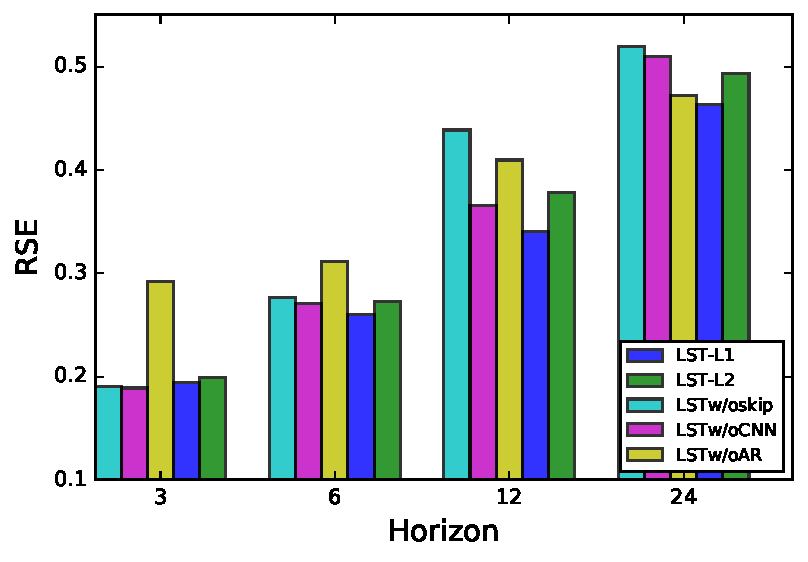
\includegraphics[width=\linewidth]{fig/rmse-solar.pdf}
    %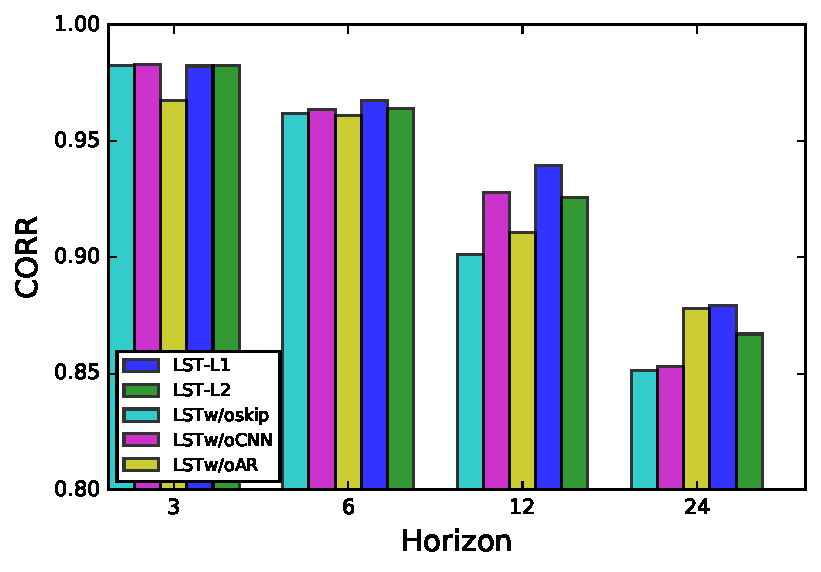
\includegraphics[width=.4\linewidth]{fig/corr-solar.pdf}
    %\vspace{-0.3 cm}
    \caption{\solar dataset}
  \end{subfigure}
  %\begin{subfigure}{.22\textwidth}
  %  \centering
  %  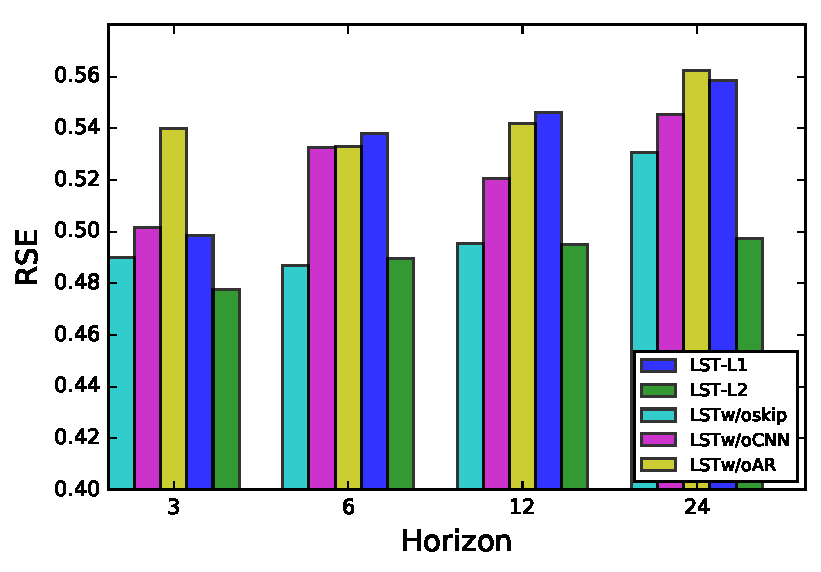
\includegraphics[width=\linewidth]{fig/rmse-traffic.pdf}
  %  %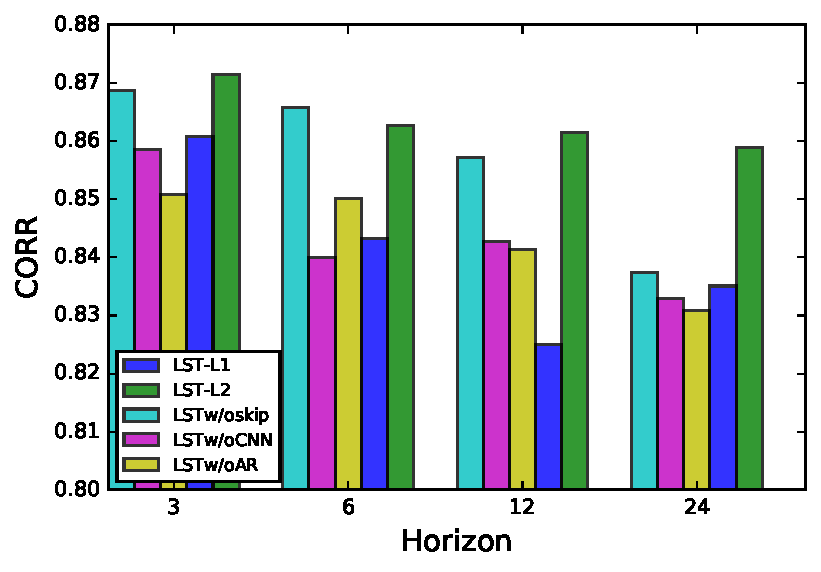
\includegraphics[width=.4\linewidth]{fig/corr-traffic.pdf}
  %  %\vspace{-0.3 cm}
  %  \caption{\traffic dataset}
  %\end{subfigure}
  \begin{subfigure}{.22\textwidth}
    \centering
    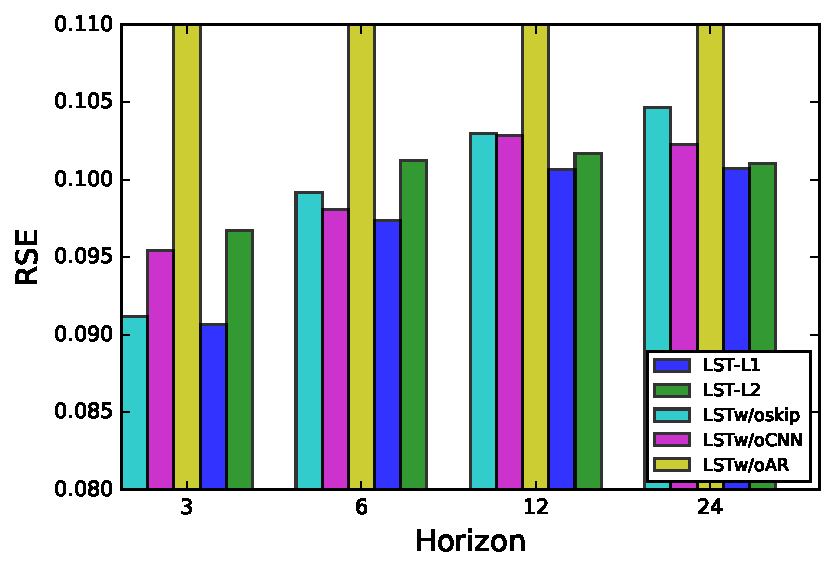
\includegraphics[width=\linewidth]{fig/rmse-ele.pdf}
    %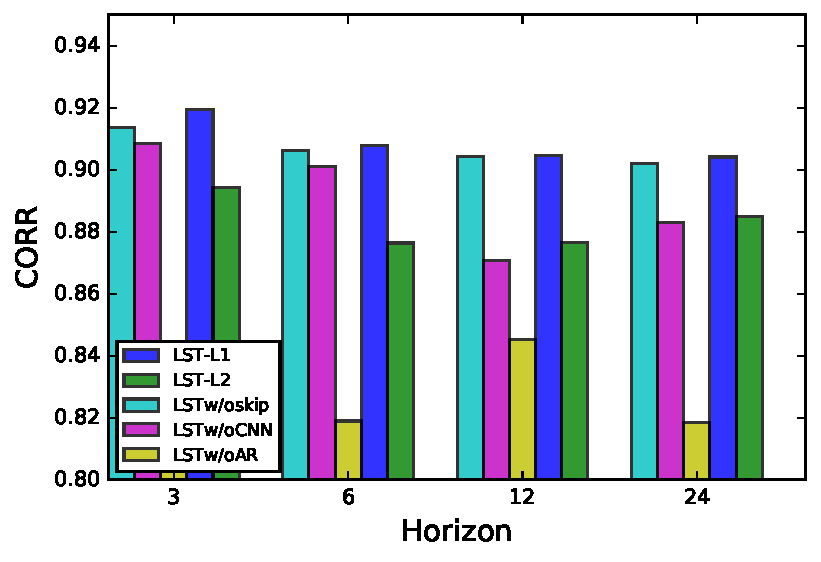
\includegraphics[width=.4\linewidth]{fig/corr-ele.pdf}
    %\vspace{-0.3cm}
    \caption{\electricity dataset}
  \end{subfigure}
  %\begin{subfigure}{.22\textwidth}
  %  \centering
  %  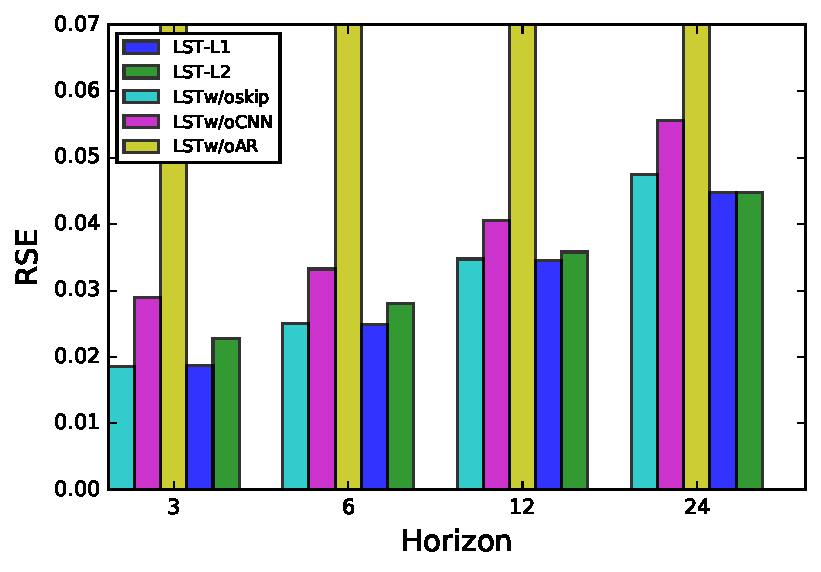
\includegraphics[width=\linewidth]{fig/rmse-exchange.pdf}
  %  %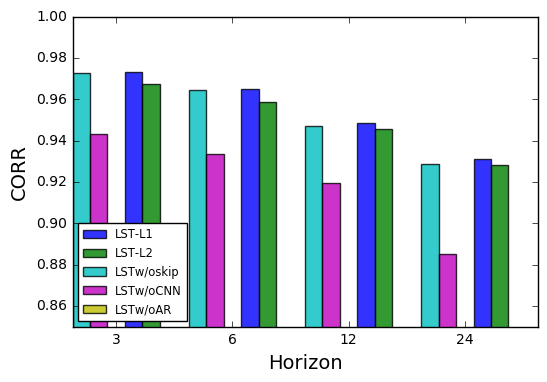
\includegraphics[width=.4\linewidth]{fig/corr-ex.png}
  %  %\vspace{-0.3 cm}
  %  \caption{\exchange dataset}
  %\end{subfigure}
  
  \caption{Results of LSTNet in the ablation tests.}
  \label{fig:ablation}
\end{figure}


\iffalse
As for why the AR component would have such an important role, our interpretation is that AR is generally robust to the sudden changes in data. To empirically validate this intuition we plot one dimension (one variable) of the time series signals in the electricity consumption dataset for the duration from 1 to 5000 hours in Figure \ref{fig:electricity}, where the blue curve is the true data and the red curve is the system-forecasted signals. We can see that the true consumption suddenly increases around the 1000th hour, and that LST-L1 successfully captures this sudden change but LSTw/oAR fails to react properly.  In other words, the neural-network component in LSTNet may not be sufficiently sensitive to random scale fluctuations in data (which is typical in \electricity data possibly due to random events for public holidays or temperature turbulence, etc.), while the simple linear AR model can make a proper adjustment in the forecasting.

\begin{figure}[!ht]
\begin{subfigure}{.23\textwidth}
  \centering
  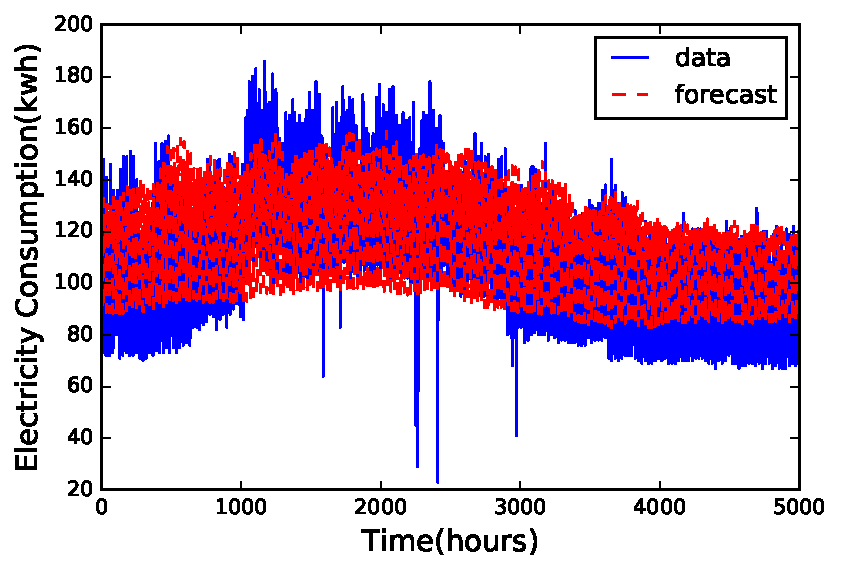
\includegraphics[width=\linewidth]{fig/woar.pdf}
  %\vspace{-0.5 cm}
  \caption{LSTNet w/o AR}
\end{subfigure}
\begin{subfigure}{.23\textwidth}
  \centering
  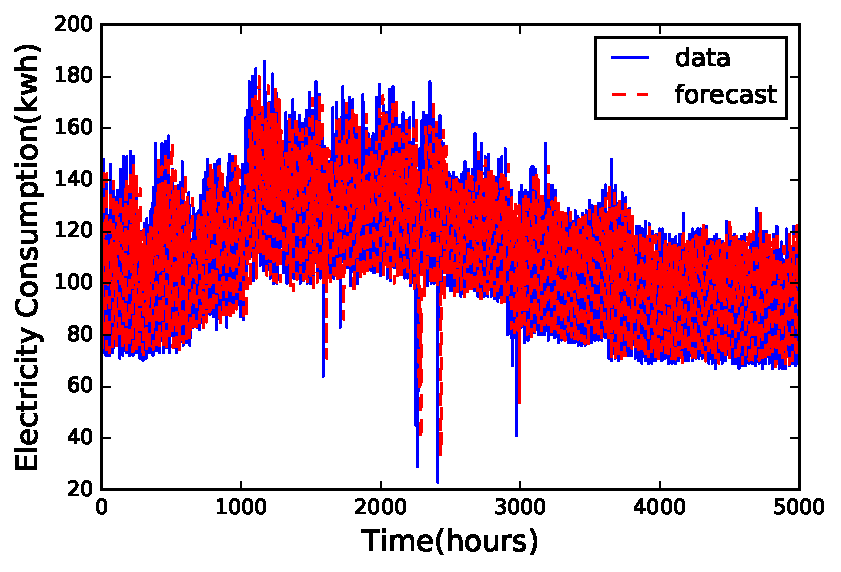
\includegraphics[width=\linewidth]{fig/war.pdf}
  %\vspace{-0.5 cm}
  \caption{LSTNet}
\end{subfigure}
\caption{The predicted time series (red) versus the true data (blue) on \electricity dataset with $horizon = 24$}
\label{fig:electricity}
%\vspace{1cm}
\end{figure}

%The LSTw/oAR fails to react very well to the fluctuated scale, and the prediction result is relatively conservative. In contrast, the complete LSTNet model can automatically adjust the prediction based on the input scale. What's more, this kind of random scale fluctuation is common in the \electricity data. One possible reason for this phenomenon is that the electricity consumption is frequently influenced by the factors hard to predict based on the history electricity consumption, e.g. the public holiday events and the temperature turbulence. However, the simple linear model adjusts the output scale according to the input by nature. After leveraging the AR component, the LSTNet structure is robust to this kind of data style. 

In summary, this ablation study clearly justifies the efficiency of our architecture design. All components have contributed to the excellent and robust performance of LSTNet.
\fi


\subsection{Mixture of long- and short-term patterns}
%\vspace{-0.1cm}
\label{sec:mixture}
To illustrate the success of LSTNet in modeling the mixture of short-term and long-term recurring patterns, Figure \ref{fig:traffic} compares the performance of LSTNet and VAR on an specific time series (one of the output variables) in the \traffic dataset. Note that the true signal (in blue) of traffic occupancy are very different on Fridays and Saturdays, and another on Sunday and Monday.

The figure shows that the VAR model is only capable to deal with the short-term patterns. The pattern of prediction results of the VAR model only depend on the day before the predictions. We can clearly see that the results of it in Saturday (2rd and 9th peaks) and Monday (4th and 11th peaks) is different from the ground truth, where the ground truth of Monday (weekday) has two peaks, one peak for Saturday (weekend). In the contrary, our proposed LSTNet model performs two patterns for weekdays and weekends respectfully. This example proves the ability of LSTNet model to memorize short-term and long-term recurring patterns simultaneously, which the traditional forecasting model is not equipped, and it is crucial in the prediction task of the real world time series signals. 
%However, the VAR model (part (a) of the figure) cannot learn such a distinction but predict the similar local patterns for both days instead. LSTNet, on the other hand (part (b) of the figure), successfully captures both the different repeating patterns on Mondays and Saturdays, and the local patterns within each day.




\begin{figure}[!ht]
  \begin{subfigure}{.23\textwidth}
    \centering
    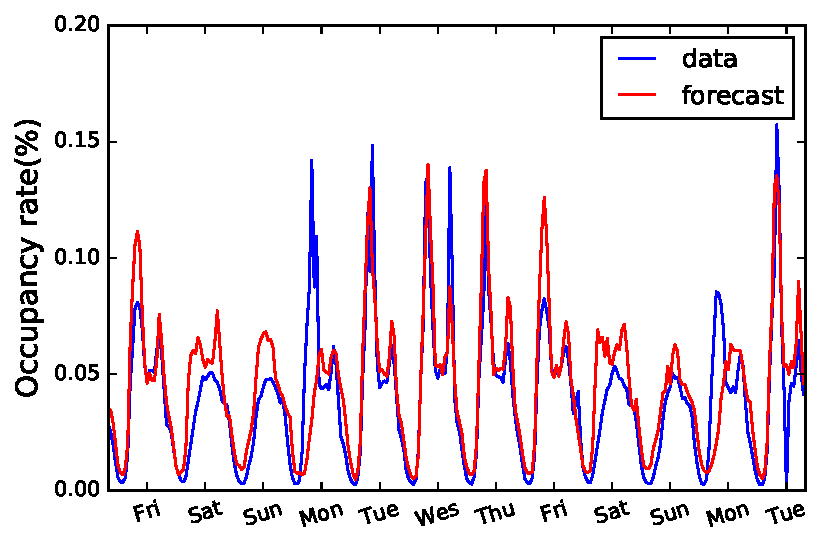
\includegraphics[width=\linewidth]{fig/traffic-var.pdf}
    \caption{VAR}
    \label{fig:tra-var}
  \end{subfigure}
  \begin{subfigure}{.23\textwidth}
    \centering
    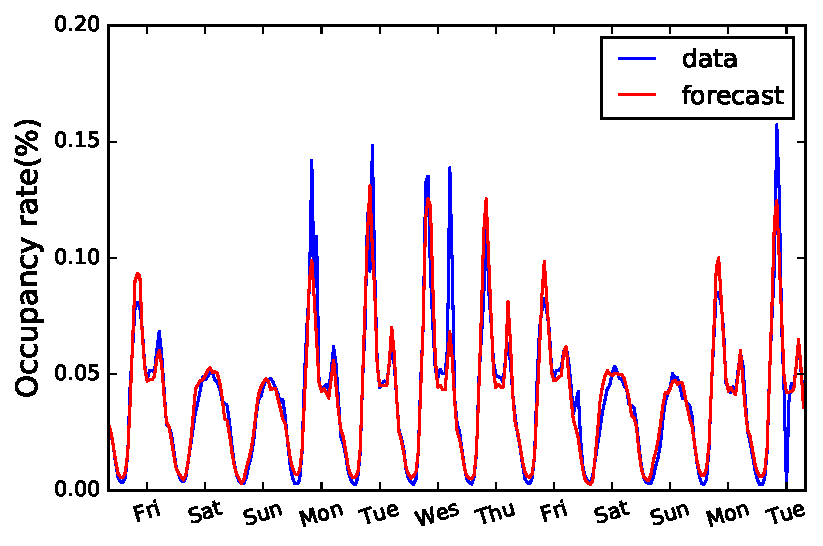
\includegraphics[width=\linewidth]{fig/traffic-tnn.pdf}
    \caption{LSTNet}
    \label{fig:tra-tnn}
  \end{subfigure}
  
  \caption{The true time series (blue) and the predicted ones (red) for one variable in the \traffic dataset. The x axis indicates the week days and the forecasting $horizon = 24$.}
  %\vspace{-0.5 cm}
  \label{fig:traffic}
\end{figure}




\section{Conclusion}
\label{sec:conclusion}
%\pagebreak
In this paper, we presented a novel deep learning framework (LSTNet) for the task of multivariate time series forecasting. By combining the strengths of convolutional and recurrent neural networks and an autoregressive component, the proposed approach significantly improved the state-of-the-art results in time series forecasting on multiple benchmark datasets. With in-depth analysis and empirical evidence we show that LSTNet indeed successfully captures both short-term and long-term repeating patterns in data, and combines both linear and non-linear models for robust prediction.  

For future research, there are several promising directions in extending the work. Firstly, the skip length $p$ of the skip-recurrent layer is a crucial hyper-parameter. Currently, we manually tune it based on the validation dataset. How to automatically choose $p$ according to data is an interesting problem. Secondly, in the convolution layer we treat each variable dimension equally, but in the real world dataset, we usually have rich attribute information. Integrating them into the LSTNet model is another challenging problem.  
%\yiming{Hanxiao: Can you add somethings here?}
%However, there are some challenges need to tackle in the future, e.g how to improve the prediction accuracy of the datasets without noticeable recurring patterns by utilizing the deep learning tools, which are prevalent in the economic activities. 

\bibliographystyle{aaai}
\bibliography{local}

\end{document}
